%% ==============================
\chapter{\iflanguage{ngerman}{Konzept}{Concept}}
\label{sec:concept}
%% ==============================
\todo{Add CommandForwarder Statepublisher}\todo{Alles noch mal lesen, und überarbeiten}
\section{Problem Statement and Goals}
As described in \autoref{c3_sec_link_ctrl_hw} the current design of \gls{r2c} is built around a \gls{sm} architecture. As a result, the control of multiple robots is only possible in two ways: 
\begin{enumerate}
    \item On one machine with tight synchronization. 
    \item On multiple machines with no significant synchronization at all.
\end{enumerate}
This has been elaborated in \autoref{c3_sec_controlling_multiple_robots} in more detail. \gls{ros2} and \gls{r2c} are developed with the goal of transferring the success of \gls{ros} to the industrial domain, where controlling multiple robots is common. The \gls{sm} approach is focused on using one computer to run the complete control stack. This approach is thereby limited in its scalability. Therefore, the main goal of this work is to test whether it is possible in the context of \gls{r2c} to run multiple controllers on multiple machines and exchange messages over \gls{dds} in a real-time like manner. This should allow a tight synchronization while unitizing multiple machines.\newline
The goal can be divided into several subordinate objectives. One is the development of a general concept for network-based communication which fits into the \gls{r2c} framework without having to change the already existing controllers and robot drivers. On the other hand, several different control architectures shall be supported. Different architectures that should be supported are for example:
\paragraph{Distributed Drivers:}\label{c4_sec_distributed_drivers}
 Distributing of controllers and drivers on different machines. Meaning, it should be possible to have for example the controller running on one computer while the drivers for communication with the hardware are running on different computers. This allows to control multiple robots with one central controller while the communication is handled by another device.
\paragraph{Distributed Chained Control:}\label{c4_sec_distributed_controller_chaining}
A central machine with a high-level controller and distributed low-level controllers on separate machines. An example for this could be a central differential drive controller on one machine and multiple PID controllers together with the drivers on multiple separate machines, for the low-level control. 


\section{Concept Overview}\label{c4_sec_overview}
In order to achieve the previously mentioned goals, a conceptual design composed of one central and multiple sub-controller managers is proposed. A schematic overview of the proposed concept is given in \autoref{c4_fig_concept_overview} and discussed in the following. It should be noted that both the central controller manager and the sub-controller managers may well manage multiple systems. For the sake of simplicity, it is focused only on the case where each sub-controller manager manages exactly one system. The central controller manager does not manage a system in this example. Moreover, in our case, the system represents a robot. One should also note, that instead of being a system, it could also be an actuator or sensor.\newline
As shown in the schematic representation \autoref{c4_fig_concept_overview}, each of the controller manager runs on its own machine. The central controller manager thereby acts as a coordinating entity, while the sub-controller managers are responsible for managing individual systems within the overall architecture.\newline
\begin{figure}[htbp]
	\centering
	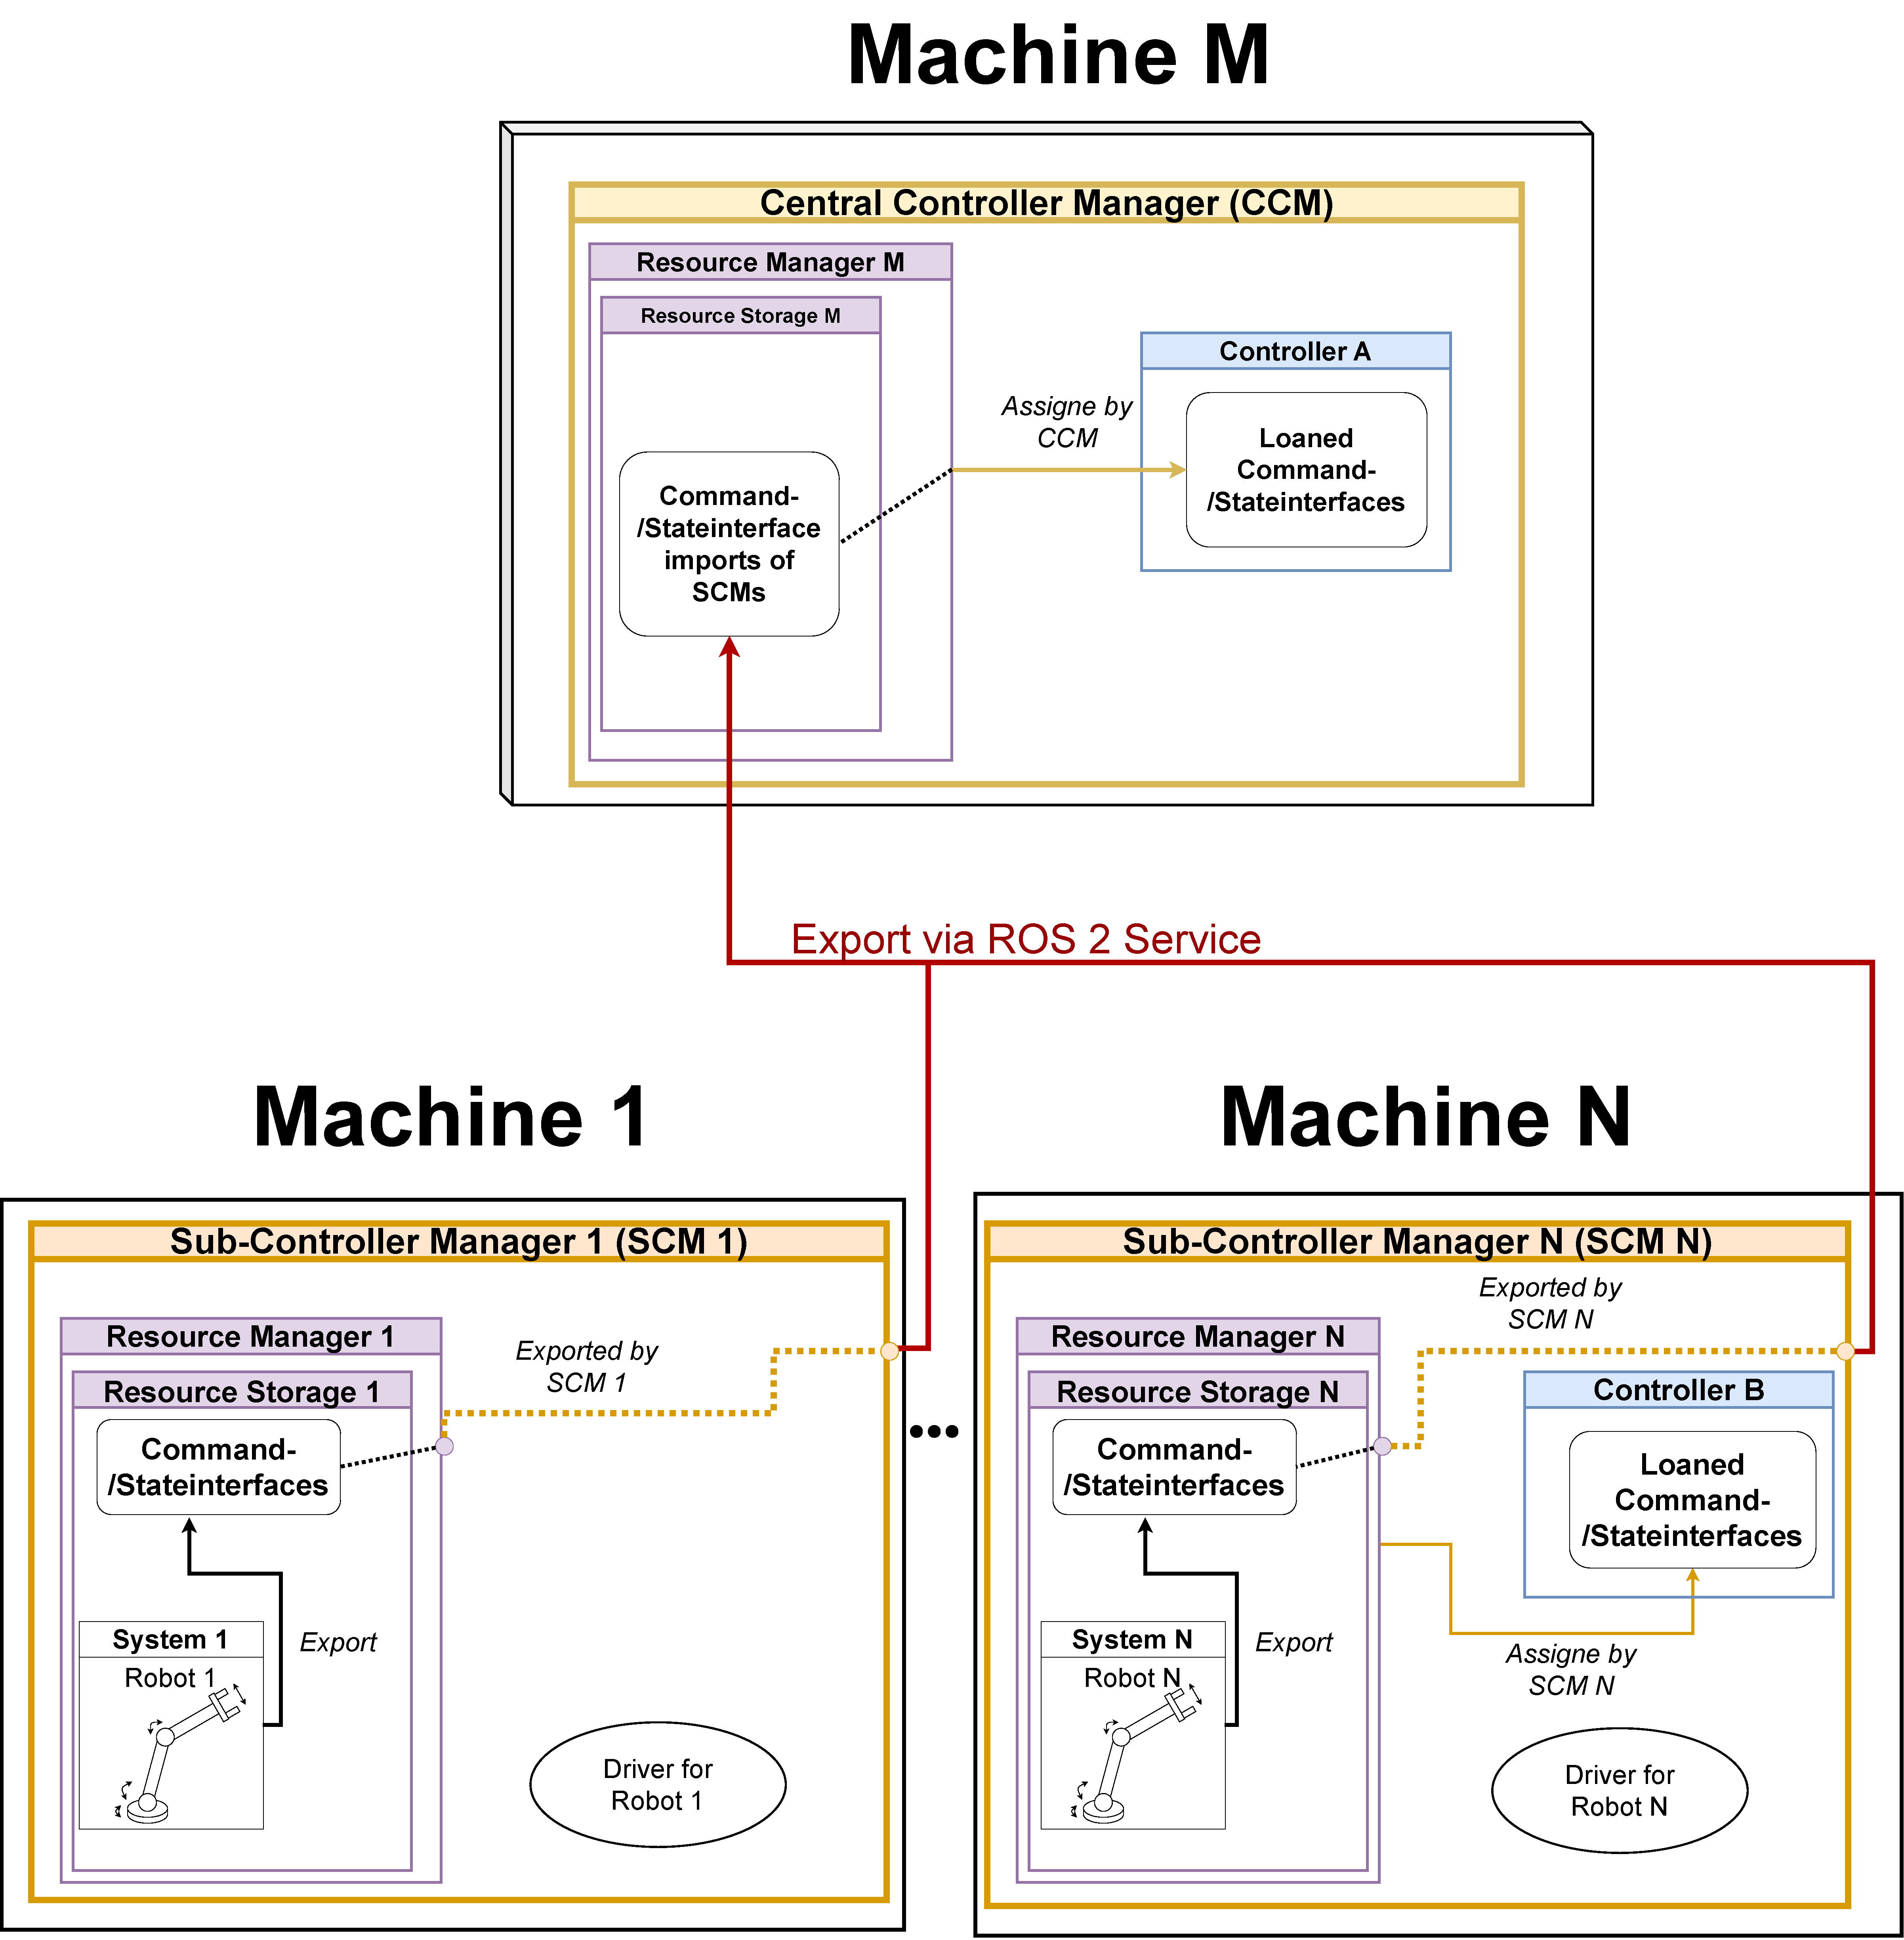
\includegraphics[width=1\textwidth]{Figures/C4/distributed_control_with_driver.pdf}
	\caption{Schematic overview of the concept implemented. The figure shows how a more complex system of multiple robots, controlled by multiple controllers on different machines, could be realized. }
	\label{c4_fig_concept_overview}
\end{figure}
\paragraph{Central Controller Manager}
The central controller manager provides services that allow sub-controller managers to register themselves with the central controller manager. The sub-controller managers then export their \glspl{ci} and \glspl{si} and create special distributed versions of them. This is indicated by the yellow dotted line inside each sub-controller manager. Those are then registered with a service call provided by the central controller manager. This is shown with the red line in the figure. With this registration service, the necessary communication between the central controller manager and the sub-controller managers are established. This way, the central controller manager facilitates the integration of multiple sub-controller managers into the system.\newline
The central controller manager can then claim the \glspl{ci} and \glspl{si}. By claiming these interfaces, the central controller manager gains access to the \glspl{ci} and \glspl{si} of the sub-controller manager's systems and can read the state and issue commands over the network as needed. This allows to run the drivers for the robots inside the sub-controller managers while the controller is running in the central controller manager on a different machine. A more detailed explanation of the necessary steps to realize this is given in \autoref{c4_sec_registraion_csi}.\newline
Alternatively, the central controller manager provides a service call for registration of \glspl{ri}. These \glspl{ri} enable the central controller manager to establish a direct connection and coordination between the controllers run by the central controller manager and controllers run by a sub-controller manager. This approach allows for chaining of controllers running on different machines.\newline
Unlike the sub-controller managers, the central controller manager does not require managing a system of its own to fulfill a useful purpose. Theoretically, a sub-controller manager could also not manage an actuator, sensor or system, but would then have no real use. In the schematic overview, this fact is illustrated with the central controller manager not having a system. The main task of the central controller manager is to coordinate and control the subordinate controller managers and their respective systems. By providing registration services, claiming interfaces, and using \glspl{ri}, the central controller manager effectively manages overall system behavior and ensures proper coordination among the sub-controller managers.
\paragraph{Sub-Controller Manager}
The sub-controller manager on the other hand is responsible for managing an individual system within the overall architecture. This is illustrated in \autoref{c4_fig_concept_overview} by the fact that each of the sub-controllers $i$ contain a corresponding system $i$. For each pair of system $i$ and system $j$, where $i\neq j$, system $i$ and system $j$ are different.\newline
Additionally, the drivers for communicating with the real hardware are then run within the context of the sub-controller managers. This means they handle low-level hardware interactions as well as controllers for higher-level control functionalities.\newline
The sub-controller managers can be configured in two ways: they can have only a driver running, or they can have both a driver and controllers running. This flexibility allows for different system setups and configurations, depending on the specific requirements of each sub-controller manager's system.
\paragraph{Limitations}
Importantly, no direct chaining of sub-controller managers is allowed within this architecture. Coordination and communication occurs exclusively between the central controller manager and each sub-controller manager. The central controller manager acts as the central point of control and coordination, orchestrating the actions of the sub-controller managers based on the state information and commands received.

In summary, the system architecture consists of a central controller manager and multiple sub-controller managers. The central controller manager provides registration services, can directly claim \glspl{ci} and \glspl{si} from the sub-controller managers, or utilize exported \glspl{ri} for controller chaining. The sub-controller managers can have either only drivers or both drivers and controllers running. Controllers can be chained inside a sub-controller manager or between sub-controller manager and central controller manager. Controller chaining inside the central controller manager is possible as well, but not between sub-controller managers.


\section{Integration in \gls{r2c}}
\subsection{New Types of \gls{ci} and \gls{si}}\label{c4_sec_adaption_of_handles}
As shown in the UML class diagram in \autoref{c3_fig_ros2_control_uml} the link between the hardware side and the controllers in the \gls{r2c} framework are the \glspl{ci} and \glspl{si}. See \autoref{c3_sec_link_ctrl_hw} for a more detailed explanation of the conceptual background. \newline
The fundamental idea of the design is to split the system at this point. Then new distributed types of \gls{ci} and \gls{si} and wrappers for the \gls{ci} and \gls{si} are introduced. Those new distributed types of handles have the same interfaces as the normal \glspl{ci} and \glspl{si} 
\begin{figure}[htbp]
	\centering
    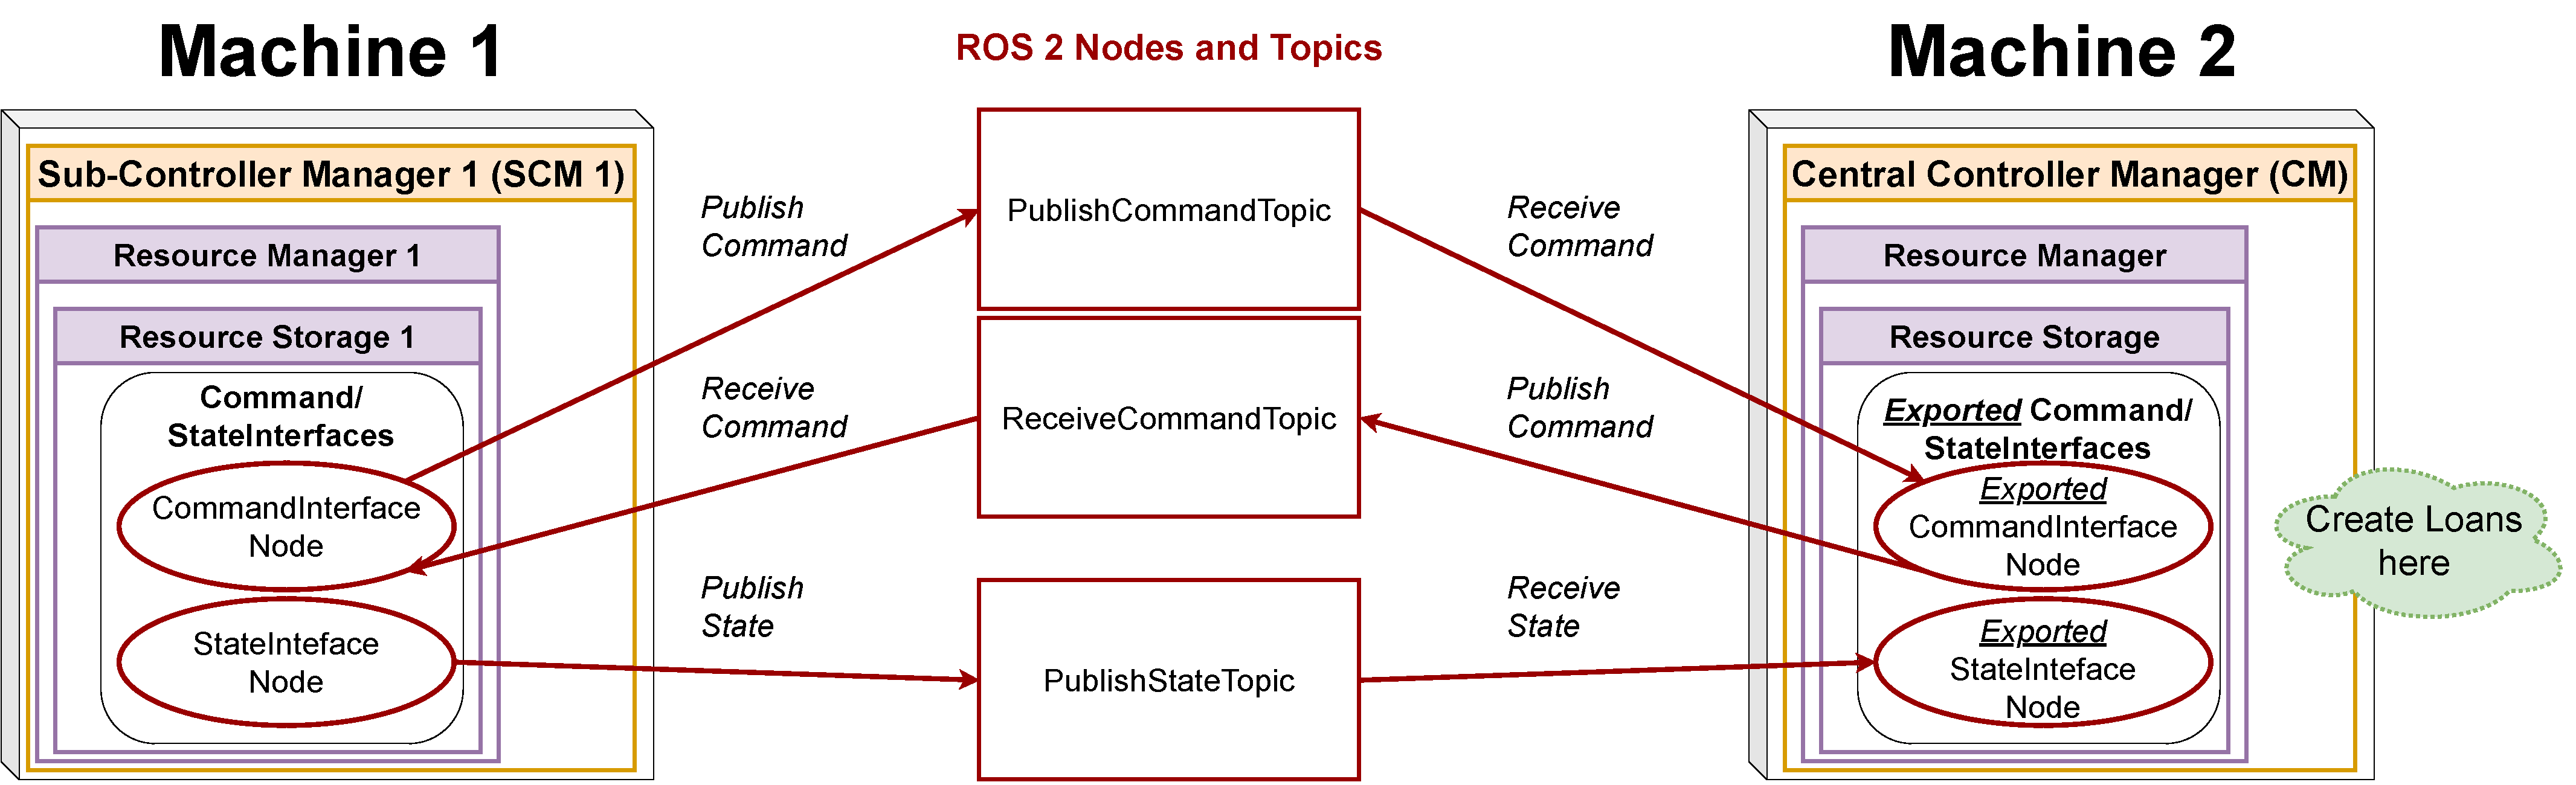
\includegraphics[width=1\textwidth]{Figures/C4/simple_concept.drawio.pdf}
	\caption{Schematic overview of how commands and states from one machine to another are transferred using topics and nodes from \gls{ros2}. The infrastructure provided by \gls{ros2} is thereby emphasized in red.}
	\label{c4_fig_simple_concept}
\end{figure}
but internally they have a \gls{ros2} node and create publishers and subscribers. This is shown in \autoref{c4_fig_simple_concept}. \newline
It has to be distinguished between the central controller manager side and the sub-controller manager side. For the central controller manager side, a distributed \gls{si} needs to receive the value, while on the sub-controller manager side the value has to be published. For distributed \glspl{ci} the same logic applies. Additionally, for writing the commands, the distributed \gls{ci} needs to publish the value set on the central controller manager's side. This command then needs to be received by the \gls{ci} on the sub-controller manager side. On the sub-controller manager side, the \glspl{ci} and \glspl{si} which should be made available for the central controller manager, are then claimed and added to a wrapper classes. Claiming of the interfaces ensures that no other controller can claim them locally and issue commands to them. The wrapper classes are needed so that the \gls{si} and \gls{ci} can remain the same. This way, the hardware drivers do not need to be changed. One type of wrapper class is needed for the \gls{si} and one for the \gls{ci}.  The wrappers are stored inside the resource storage of the sub-controller manager. Further, the wrapper classes then publish the state of the \glspl{ci} and \glspl{si}, as well as receive the commands for the \glspl{ci}. On the central controller side the new types of distributed interfaces are created which act as counterparts to the wrapper classes on the sub-controller manager side. As can be seen in \autoref{c4_fig_simple_concept}, the new types of \glspl{ci} and \glspl{si} on the central controller manager's side are stored inside the \textit{ResourceStorage} as normal \glspl{ci} and \glspl{si} are.\newline 
The information of what distributed \glspl{ci} and \glspl{si} and which publishers and subscribers should be created is made available with the registration. The registration process and what is created, stored and managed where is explained in more detail in the following sections.

\subsection{Conceptual Registration of a Sub-Controller Manager}\label{c4_sec_registraion_csi}
The registration of a sub-controller manager at a central controller manager involves a series of steps and actions. Those actions are performed by both the sub-controller manager and the central controller manager. This is needed in order to establish the aforementioned connection between the distributed \glspl{ci} and \gls{si} of the central controller manager and the wrapper classes of the sub-controller manager.

First, the conceptual steps the central controller manager needs to do in order to establish connection are explained:
\begin{enumerate}
    \item Create a service for registration. The central controller manager creates a service that allows sub-controller managers to initiate the registration process. This service acts as an interface for receiving registration requests. The request should thereby have the name and namespace of the sub-controller manager, as well as the names of the topics created by the wrapper classes of the \glspl{ci} and \glspl{si}. 

    \item Register the sub-controller manager upon receiving a registration call. When a registration call is received, the central controller manager should then create a special wrapper object for the sub-controller manager's request and store the corresponding information. This involves e.g. adding the sub-controller manager's name to its list of managed components.

    \item Create the distributed \glspl{ci} and \glspl{si} of the wrapped \glspl{ci} and \glspl{si} of the sub-controller manager. These distributed \glspl{ci} and \glspl{si} should then subscribe to publishers of the wrappers of the sub-controller manager. After a successful subscription and creation of the distributed interfaces, they are stored inside the central controller manager's \textit{ResourceManager} as \glspl{ci} and \glspl{si}. This allows the central controller manager to receive updates about the commands and state information from the sub-controller manager. At the same time, those distributed \glspl{ci} and \glspl{si} can then be claimed by controllers of the central controller manager.

    \item As a next step, the central controller manager needs to create publishers for each of the received wrapper of a \glspl{ci}. This is needed to issue commands to the sub-controller manager's \glspl{ci}. As \glspl{si} are only unidirectional, nothing needs to be done here. 
    
    \item The last step is then to send the topic names of those created publishers back to the sub-controller manager. This is done with the response of the provided service. 

    \item From here on, the central controller manager can then proceed as normal. All the necessary connections are established. If the \glspl{ci} and \gls{si} are then claimed within the central controller manager, nothing special needs to be done, since the interface for accessing the state and issue commands stays the same. The controller claiming the distributed handles is not aware that the data received by the \glspl{si} is in fact sent over the network. The same holds true for commands issued by the controller. The controller can then write its command to the distributed \glspl{ci} and the sending over the network is handled internally.
\end{enumerate}

The sub-controller manager needs to perform the following tasks during the registration process:
\begin{enumerate}
    \item For each of the available \glspl{ci} and \glspl{si} claim the interface and create loans. Then those loans are added to wrapper classes.  Those are then stored in the \textit{ResourceStorage}. The wrapper classes are internally creating publishers and the names of those topics are then stored. The states of the \glspl{si} and \glspl{ci} are then published on the created topics.

    \item The sub-controller manager needs then to register at the central controller manager. In the registration call, the namespace, name as well as the names of the topics for wrappers of the \glspl{ci} and \glspl{si} are included. 
    
    \item Wait for registration to successfully complete. 
    
    \item With the response, the sub-controller manager receives the names of the topics for the central controller manager's distributed \glspl{ci}. The sub-controller manager then needs to update it the wrappers for the \glspl{ci} stored in the \textit{ResourceStorage}. This needs to be done, so that they can subscribe to the topics of the central controller manager's distributed \gls{ci}. This allows the sub-controller manager to receive commands from the central controller manager and issue them to the hardware via the driver.

    \item Once all the necessary connections and subscriptions are established, the sub-controller manager can operate normally. On the driver site of the \gls{r2c} framework no change is needed this way. A driver exports its \glspl{ci} and \glspl{si} as it would normally. The creation of the topics and the handling of the subscription is done in the sub-controller manager internally. A driver can read the commands from the \gls{ci} as normal and does not know or need to know that the command was received over the network.
    
\end{enumerate}
Overall, the described conceptual registration process between the sub-controller manager and the central controller manager involves establishing connections via a service call, creating of publishers and subscribers, and ensuring communication between the components this way. This is all done while the already existing controllers and drivers of the framework can stay the same and don't need to be updated.

\subsection{Distributed Controller Chaining}
Our second sub goal regarding decentralized control includes the necessity to chain the input of a sub-controller manager's controller to the output of a controller that is running on a different machine. In order to make it possible to chain controllers of a sub-controller manager and a central controller manager, a few steps have to be done. The conceptual procedure of how to chain the controller in a distributed manner over the network are described in the following.

First, the steps and actions which the central controller manager needs to perform are presented:
\begin{enumerate}
    \item Create a service for registration. The central controller manager creates a service that allows sub-controller managers to register the \glspl{ri}. The request should thereby have the name and namespace of the sub-controller manager, as well as the names of the topics created by the wrapper of the \glspl{ri}.
        
    \item Upon receiving a request from a sub-controller manager to register its \glspl{ri} the central controller manager checks its stored components for the sub-controller manager. The central controller manager then imports the description of the \glspl{ri} provided by the sub-controller managers. It then creates distributed \glspl{ci}. In a first step, the \glspl{ci} subscribes to the topic provided by the wrapper of the \glspl{ri}. In a second step, the distributed \glspl{ci} need to create topics themselves.
    
    \item Next, create the response for the service call and add the topic names for the created distributed \gls{ci} to it. The response is then sent back to the sub-controller manager.
    
    \item  Once the description of the \glspl{ri} are imported and the distributed \glspl{ci} are created, the central controller manager can continue its regular operations. A controller of the central controller manager can then claim those \glspl{ci} and issue commands to them, which are then sent over the network to the \glspl{ri} of the sub-controller manager's controllers.
\end{enumerate}

The sub-controller manager performs the following tasks to facilitate the chaining of controllers:
\begin{enumerate}
    \item The chained mode of the sub-controller manager's controllers is enabled. The controller no longer receives its input from subscriptions or services. It creates \glspl{ci}, which in the context of chained controllers are called \glspl{ri}. Those \glspl{ri} are then exported and added to the \textit{ResourceStorage} of the sub-controller manager.

    \item The sub-controller manager then claims the \glspl{ri} and creates loans. The loans are the wrapped inside a wrapper class and the wrapper class is stored in the \textit{ResourceStorage}. The wrapper class creates topics on which the stored value of the \gls{ci} is published on.
        
    \item In a next step, the sub-controller manager initiates the registration process by calling the central controller manager's service. Beside the namespace and name, the topic names of the \glspl{ri} are added to the request.

    \item Upon successful registration, the sub-controller manager receives the topic names of the central controller manager's distributed \glspl{ci} for the \glspl{ri}. The wrapper classes of the \glspl{ri} are then subscribed to those topics.

    \item The registration procedure is complete. Now, a connection between the controller of the central controller manager and the controller of the sub-controller manager is established. The sub-controller manager can proceed with its normal operation.

\end{enumerate}
In summary, the conceptual registration process and chaining of controllers between the sub-controller manager and the central controller manager involves registration of the \glspl{ri} created by a controller of the sub-controller manager. Further, a connection between the output of the central controller managers controller and the input of the sub-controller managers controller is established. This allows for chaining of controllers running on different machines. Moreover, with the proposed procedure, the controllers as well as the process for chaining and exporting of \glspl{ri} can stay the same and no changes need to be done.
\missingfigure{vllt ablauf diagram für registraion}
\missingfigure{vllt ablauf diagramm für reference.}